\section{Cluster Performance}


\subsection{Size of Cluster}
For a fixed size input, show how adding more workers changes the running time

Not too sure how it will work with pure hadoop stuff as giraph can choose the number of workers to use

\subsubsection{Enron}
Using the Enron dataset as fixed size input, we are hoping to show that as the number of workers increase, the runtime of the algorithms decrease. From observations, the PageRank algorithm has shown to be one of the more time consuming algorithms, and as such has been chosen to perform analysis of the cluster.

\begin{figure}[htbp]%
\centering
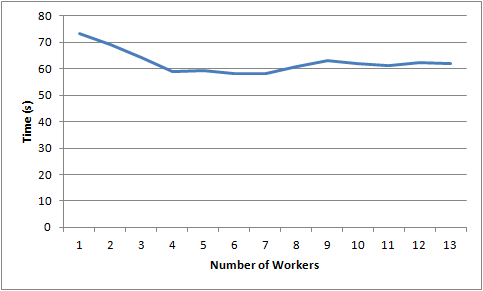
\includegraphics[]{./img/pagerank-enron-benchmark}%
\caption{Runtime of PageRank algorithm on Enron dataset with varying number of workers}%
\label{fig:enronbenchmark}%
\end{figure}

Figure \ref{fig:enronbenchmark} shows the running time of the PageRank algorithm on the Enron dataset consisting of 36692 nodes and 367662 edges. As expected, the running time of the algorithm initially decreases quite rapidly as the number of workers increases up to a fourth worker. There is minimal decrease in running time from the fourth to the seventh worker, followed by a jump after an eight worker is added. After this, the number of workers added do not affect the running time of the algorithm.

The longest running time, as to be expected, was with one worker. The shortest running time was with seven workers, again this is possibly to be expected as the cluster is in operation with seven slave nodes, so each node has an equal but small share of the original network. The running time does not decrease much from four to seven workers, most likely due to the increased network costs of having these extra workers offsetting the decrease in running time each worker will have from having less nodes to process.

After an eight worker is included, the running time then increases and stabilises just above the sixty second mark. This is most likely due to the nodes requiring to launch extra processes for the extra workers, which slows down the execution of workers on nodes with more than one worker.

\subsection{Size of Input}
For a fixed number of workers, show how changing the input size affects the running time